\documentclass[11pt]{article}

\usepackage{amsmath}
\usepackage{amsfonts} 
\usepackage{amsthm}
\usepackage{caption}
\usepackage{enumitem} 
\usepackage{soul}
\usepackage{mathtools}
\usepackage{clrscode3e}
\usepackage{graphicx}
\usepackage{tikz}
\usetikzlibrary {arrows.meta,bending}
\usepackage[top=2cm,bottom=2cm,left=1.5cm,right=2cm,marginparwidth=1.75cm]{geometry}
\setlength{\parindent}{0cm}

\newcommand{\R}{\mathbb{R}}
\newcommand{\n}{\vspace{0.5cm}}

\def\lc{\left\lceil}   
\def\rc{\right\rceil}
\def\lf{\left\lfloor}   
\def\rf{\right\rfloor}

\newtheorem{theorem}{Theorem}

\pagenumbering{gobble}
\title{\vspace{-1.0cm}\textbf{CSCI 5103 Assignment 2}}
\date{February 10, 2023}
\author{\textbf{Fletcher Gornick}\\(x500: gorni025, ID: 5579904)}

\begin{document}
\maketitle

\begin{enumerate}
  \item Suppose that it takes 15 milliseconds of CPU to get a request for work, dispatch it, and do the rest of the necessary processing, assuming that the data needed are in the main memory.  If a disk storage server operation is needed, as is the case for \ul{one-third of the requests}, an additional 75 millisecond is required, during which time the thread sleeps.
    \begin{enumerate}
      \item How many requests per second can this server handle if it is single-threaded? \n\\
        Every \(1/3\) requests will take \(15+75=90\) ms of CPU time, and 15 ms for the other \(2/3\) times, so on average it takes \(\frac{15 + 15 + 90}{3} = 40\) ms to complete one request.  This means the single-threaded server should be able to handle \(\frac{1000}{40} = \textbf{25}\) requests per second. \n

      \item How many requests per second can this web-server handle if it is multi-threaded?  Assume that the storage server handles the requests \ul{sequentially} and for each request it takes 75 milliseconds to complete the I/O. \n\\
        In this case, whenever a thread sleeps to wait for I/O, we can simply switch to a different thread, so each request takes 15 ms.  There is still the case where the last thread scheduled will need to fully complete I/0, so we do need to account for the last 75ms of lost time. \\
        This results in \(\frac{1000 - 75}{15} = \textbf{61.67}\) requests per second.\n

      \item Now consider a system with a slightly different kind of high performance storage system.  Assume that this storage server can handle any number of requests concurrently and each I/O request completes in 75 milliseconds.  How many service requests per second can this web server handle if it is multi-threaded? \n\\
        For the last case, we can context switch the threads whenever, so with a good enough scheduler, we never need to waste CPU time waiting for I/O.  This means we should be able to handle \(\frac{1000}{15} = \textbf{66.67}\) requests per second. \n
    \end{enumerate}
    \newpage

  \item Consider a system with a single CPU server in which jobs arrive at rate \(\textbf{A}\) jobs per unit time.  Each job requires average \(\textbf{S}\) units of CPU time.  Assume that the jobs arrive at \ul{random points in time}.  Moreover, assume that jobs are processed using the \ul{FCFS scheduling policy}.  There are no I/O operations involved in processing a job.
    \begin{enumerate}
      \item What is the CPU utilization, denoted by \(\textbf{U}\) in this system?  Express \(\textbf{U}\) in terms of \(\textbf{A}\) and \(\textbf{S}\). \n\\


      \item Let the random variable \(X\) denote the number of jobs already present in the system when a new job arrives.
        \begin{enumerate}
          \item What is \(P(X=0)\)? This is the probability that a new arriving job finds the system idle. \n\\
            CPU utilization \(\textbf{U} = 1 - P(X=0)\), so \(P(X=0) \)\n

          \item What is the \(P(X>0)\)?  This is the probability that a new arriving job finds the system busy. \n\\
            CPU utilization \(\textbf{U} =\) P(CPU busy), so \(P(X>0) = U\)\n
        \end{enumerate}

      \item Let \(N\) denote the average number of jobs in this system and let \(T\) be the average turnaround time, i.e. the average amount of time a job spends in the system, starting from the instant when it enters the system to the point in time when it departs.  

        (\(N\) is also the average value of the random variable \(X\).  Given that jobs arrive at random points in time, a newly arriving job would find the average number of jobs in the system equal to \(N\). Also, by \textit{Little's Law}, \(N = AT\).)  \textbf{What is the relationship between \(W\), \(N\) and \(U\)}?

      \item With \ul{FCFS job scheduling discipline}, an arriving job has to wait for the completion of all of the jobs before it in the system.  \textbf{\ul{Ignoring}} the amount of service a job in the system may have already received, and assuming that each of these jobs would still require \(S\) units of service-time, \textbf{give an expression for the average turnaround time T in terms of \(S\), \(U\) and \(N\)}.

      \item Using Little's Law, which says \(N=AT\), and the results from the part (d) above, \textbf{derive an expression for \(N\) in terms of the server utilization \(U\)}.
    \end{enumerate}
    \newpage

  \item Consider a real-time system consisting of two periodic tasks.  Assume these tasks only require the CPU and do not perform any I/O.  Task A has a period of 50 seconds and requires 25 seconds of CPU time.  Task B has a period of 70 seconds and requires 28 seconds of CPU time.
    \begin{enumerate}
      \item Is the condition for \ul{Rate Monotonic} (RM) scheduling satisfied? \n
        \[\frac{25}{50} + \frac{28}{70} = 0.9 > 0.828 = 2(2^{1/2} - 1),\] 
        so \textbf{the condition for Rate Monotonic scheduling is NOT satisfied.} \n

      \item Is a schedule possible using RM-based static priorities? If yes, \ul{show a schedule}.  Otherwise, \ul{show a case} where any of these two tasks misses its deadline. \n
        \begin{center}
          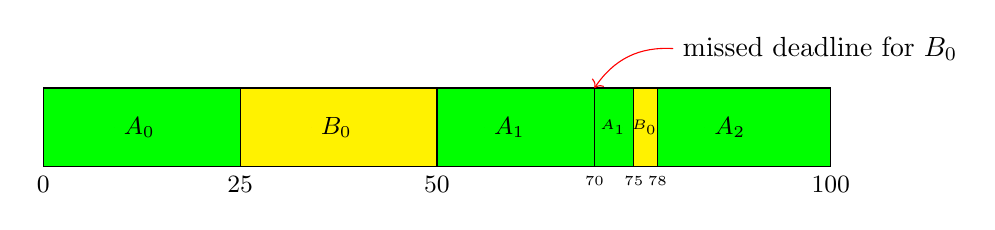
\begin{tikzpicture}
            \filldraw[color=black, fill=green] (0,0) rectangle (2.5,1);
            \filldraw[color=black, fill=yellow] (2.5,0) rectangle (5,1);
            \draw[color=black, fill=green] (5,0) rectangle (7,1);
            \draw[color=black, fill=green] (7,0) rectangle (7.5,1);
            \draw[color=black, fill=yellow] (7.5,0) rectangle (7.8,1);
            \draw[color=black, fill=green] (7.8,0) rectangle (10,1);

            \filldraw[black] (0,0) circle (0pt) node[anchor=north]{\small 0};
            \filldraw[black] (2.5,0) circle (0pt) node[anchor=north]{\small 25};
            \filldraw[black] (5,0) circle (0pt) node[anchor=north]{\small 50};
            \filldraw[black] (7,0) circle (0pt) node[anchor=north]{\tiny 70};
            \filldraw[black] (7.5,0) circle (0pt) node[anchor=north]{\tiny 75};
            \filldraw[black] (7.8,0) circle (0pt) node[anchor=north]{\tiny 78};
            \filldraw[black] (10,0) circle (0pt) node[anchor=north]{\small 100};

            \filldraw[black] (0.9,0.5) circle (0pt) node[anchor=west]{\small \(A_0\)};
            \filldraw[black] (3.4,0.5) circle (0pt) node[anchor=west]{\small \(B_0\)};
            \filldraw[black] (5.6,0.5) circle (0pt) node[anchor=west]{\small \(A_1\)};
            \filldraw[black] (6.95,0.5) circle (0pt) node[anchor=west]{\tiny \(A_1\)};
            \filldraw[black] (7.35,0.5) circle (0pt) node[anchor=west]{\tiny \(B_0\)};
            \filldraw[black] (8.4,0.5) circle (0pt) node[anchor=west]{\small \(A_2\)};

            \draw [red] (8,1.5) [->] to [bend right] (7,1);
            \filldraw[black] (8,1.5) circle (0pt) node[anchor=west]{missed deadline for \(B_0\)};
          \end{tikzpicture}
        \end{center}

      \item Suppose we upgrade the CPU to be 25\% more powerful than the original, i.e., the power of the new CPU is 1.25 times that of the original.  Is the RM scheduling condition satisfied with this new configuration?  Keep in mind that that this does not change the task recurrence periods. \n
        Since the CPU is 25\% more powerful, so the CPU time for task \(A\) is now \(25/1.25 = 20\), and for task \(B\), it's now \(28/1.25 = 22.4\).  So we can check these new values for our RMS constraint:
        \[\frac{20}{50} + \frac{22.4}{70} = 0.72 < 0.828 = 2(2^{1/2} - 1),\] 
        so \textbf{the condition for Rate Monotonic scheduling IS satisfied.} \n

      \item Answer question (b) above with the configuration given in (c). \n
        \begin{center}
          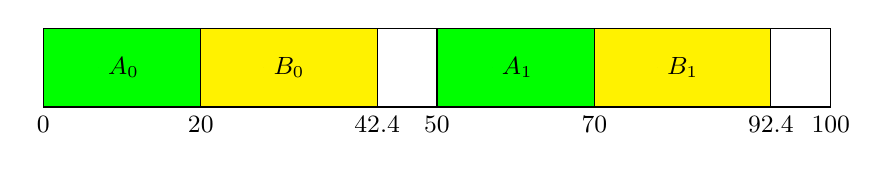
\begin{tikzpicture}
            \filldraw[color=black, fill=green] (0,0) rectangle (2,1);
            \filldraw[color=black, fill=yellow] (2,0) rectangle (4.24,1);
            \draw (4.24,0) rectangle (5,1);
            \filldraw[color=black, fill=green] (5,0) rectangle (7,1);
            \filldraw[color=black, fill=yellow] (7,0) rectangle (9.24,1);
            \draw (9.24,0) rectangle (10,1);

            \filldraw[black] (0,0) circle (0pt) node[anchor=north]{\small 0};
            \filldraw[black] (2,0) circle (0pt) node[anchor=north]{\small 20};
            \filldraw[black] (4.24,0) circle (0pt) node[anchor=north]{\small 42.4};
            \filldraw[black] (5,0) circle (0pt) node[anchor=north]{\small 50};
            \filldraw[black] (7,0) circle (0pt) node[anchor=north]{\small 70};
            \filldraw[black] (9.24,0) circle (0pt) node[anchor=north]{\small 92.4};
            \filldraw[black] (10,0) circle (0pt) node[anchor=north]{\small 100};

            \filldraw[black] (0.7,0.5) circle (0pt) node[anchor=west]{\small \(A_0\)};
            \filldraw[black] (2.8,0.5) circle (0pt) node[anchor=west]{\small \(B_0\)};
            \filldraw[black] (5.7,0.5) circle (0pt) node[anchor=west]{\small \(A_1\)};
            \filldraw[black] (7.8,0.5) circle (0pt) node[anchor=west]{\small \(B_1\)};
          \end{tikzpicture}
        \end{center}
    \end{enumerate}
    \newpage

  \item The following solution to the \ul{two-process critical section problem} was presented in 1966, and later this solution was found to be incorrect.  \textbf{Give an example to show how the mutual exclusion requirement is violated}.

    (You \textbf{\ul{MUST show}} an interleaved execution of the steps of these two processes, leading to the violation of the mutual exclusion requirement.  Indicate line numbers for steps when showing an interleaved execution of the two processes violating the mutual exclusion requirement.) \n

    The two processes are numbered 0 and 1. \\
    The shared variables are: \\
    \hspace*{1cm} var flag: array[0..1] of boolean /* initially false */ \\
    \hspace*{1cm} turn: 0..1; /* assume any initial value */

    \begin{codebox}
     \Procname{\(\proc{Process (i)}\)}
     \zi /* i can either 0 or 1, j is (i+1) mod 2 */
     \li repeat \Do
        \zi // ENTRY PROTOCOL
        \li flag[i] = true;
        \li \While (turn != i) do \{\Do
          \li \While (flag[j]) do /* nothing */;
          \li turn = i;
        \End
        \li \}
        \li CRITICAL SECTION
        \zi // EXIT PROTOCOL
        \li flag[i] = false;
        \li \(\hdots\)
     \End
     \li until false;
    \end{codebox}
    \newpage

  \item \textit{\ul{Definition (Counting Semaphore)}}: A semaphore that can have any arbitrary positive integer value, including value 0.  A signal operation increases the value by 1 if there is no waiting process.

    \textit{\ul{Definition (Binary semaphore)}}: A semaphore that can have values only 0 or 1; a signal operation has no effect if the value is already 1. \n

    You are asked to \ul{show how to implement a \textit{counting semaphore} using \textit{binary semaphores}}.  In your implementation, in addition to using binary semaphores, you may use additional data items such as integer counters or Boolean flags.

    You have to show implementations of \ul{wait} and \ul{signal} operations of the counting semaphore.

    \textit{(Hint: You can use a binary semaphore with initial value 1 to implement a critical section.  For maintaining a queue of blocked processes, you can use a binary semaphore with initial value 0.)}
    \newpage

  \item \textit{Barrier synchronization problem}: A parallel program contains \(N\) processes, which execute in synchronized phases (steps).  After completing the execution of phase i, each process waits for all the other processes to complete their i’th phase. For this purpose, after executing the code for phase i, each process executes a function called \textit{BarrierSynch(i)}.  When the last process reaches the barrier and executes this synchronization function, it unblocks all the other (\(N-1\)) waiting processes to resume their execution for phase (i+1). This form of execution of steps and barrier synchronization repeats at each phase.

    Write synchronization code for the function \textit{BarrierSynch(phase-number)} using \textbf{\ul{semaphores}} and any other shared variables to implement the barrier synchronization problem described above.  (\ul{Important}: You should pay attention to \ul{race conditions} where a process resumed from i’th phase barrier may quickly finish its execution of the next phase and start executing the barrier synchronization code of function for the (i+1)’th phase while some other processes are still executing the barrier synchronization code for phase i.)

    \begin{center}
      \includegraphics[width=0.7\textwidth]{barrier-sync.png}
    \end{center}
    \newpage
    
  \item Suppose a system has \ul{two producer processes} \(P_1\) and \(P_2\), and one consumer process \(C_1\).  All these three processes execute concurrently, and possibly at different speeds.  This system contains a shared buffer of length \(2N\) slots for communicating items between the producers and the consumer.  An item consists of two parts, \(I_1\) and \(I_2\) which are produced by \(P_1\) and \(P_2\) respectively, i.e. \(P_1\) produces parts of type \(I_1\), and \(P_2\) produces parts of type \(I_2\).  Each part occupies one slot in the buffer, allowing for \(N\) items to exist in the buffer.  The two types of parts must occupy alternating positions in the buffer, and always appear in the same order such as \(I_1\) followed by \(I_2\).  \ul{The consumer always removes a complete item}, i.e. one part of type \(I_1\) and the other of type \(I_2\), from the buffer.

    \ul{Using semaphores, write pseudo-code of these three processes to synchronize the producers and consumer in this system}.

    Figure below shows \textbf{\ul{an example}} of possible contents of a buffer of length 8.

    \begin{center}
      \scalebox{2}{
        \begin{tabular}[c]{|l|l|l|l|l|l|l|l|}
          \hline
          \(I_1\) & \(I_2\) & \(I_1\) & \(I_2\) & \(I_1\) & \(\;\;\) & \(I_1\) & \(\;\;\) \\
          \hline
        \end{tabular}
      }
    \end{center}
    \newpage

  \item Write a \ul{monitor} called \textit{Aggregator} with one interface procedure named \textit{Add(integer n)}, which will be used by three asynchronous processes as described below.

    Each process will have some integer number \(n\), which it will report to the \textit{Aggregator} by calling its interface procedure \textit{Add(n)}.  This monitor method will return the sum of the three integer values reported by these three processes after all have reported their values.

    When a process calls \textit{Add(n)} and if the other two processes haven’t yet reported their values, the execution of this procedure will get suspended.  This execution will resume when all three values have been reported and the sum of these values can be returned as the return value of \textit{Add(n)}.
    
\end{enumerate}
\end{document}
